%!TEX TS-program = xelatex  
\documentclass[12pt,a4paper]{article}

\usepackage{etex} % расширение классического tex в частности позволяет подгружать гораздо больше пакетов, чем мы и займёмся далее

%%%%%%%%%% Математика %%%%%%%%%%
\usepackage{amsmath,amsfonts,amssymb,amsthm,mathtools} 
%\mathtoolsset{showonlyrefs=true}  % Показывать номера только у тех формул, на которые есть \eqref{} в тексте.
%\usepackage{leqno} % Нумерация формул слева


%%%%%%%%%%%%%%%%%%%%%%%% Шрифты %%%%%%%%%%%%%%%%%%%%%%%%%%%%%%%%%
\usepackage{fontspec}         % пакет для подгрузки шрифтов
\setmainfont{Arial}   % задаёт основной шрифт документа

\defaultfontfeatures{Mapping=tex-text}

% why do we need \newfontfamily:
% http://tex.stackexchange.com/questions/91507/
\newfontfamily{\cyrillicfonttt}{Arial}
\newfontfamily{\cyrillicfont}{Arial}
\newfontfamily{\cyrillicfontsf}{Arial}

\usepackage{unicode-math}     % пакет для установки математического шрифта
\setmathfont{Asana Math}      % шрифт для математики

\usepackage{polyglossia}      % Пакет, который позволяет подгружать русские буквы
\setdefaultlanguage{russian}  % Основной язык документа
\setotherlanguage{english}    % Второстепенный язык документа


%%%%%%%%%% Работа с картинками %%%%%%%%%
\usepackage{graphicx}                  % Для вставки рисунков
\usepackage{graphics} 
\graphicspath{{Pics/}}    % можно указать папки с картинками
\usepackage{wrapfig}                   % Обтекание рисунков и таблиц текстом
\usepackage{subfigure}                 % для создания нескольких рисунков внутри одного


%%%%%%%%%% Работа с таблицами %%%%%%%%%%
\usepackage{tabularx}            % новые типы колонок
\usepackage{tabulary}            % и ещё новые типы колонок
\usepackage{array}               % Дополнительная работа с таблицами
\usepackage{longtable}           % Длинные таблицы
\usepackage{multirow}            % Слияние строк в таблице
\usepackage{float}               % возможность позиционировать объекты в нужном месте 
\usepackage{booktabs}            % таблицы как в книгах!  
\renewcommand{\arraystretch}{1.3} % больше расстояние между строками


\usepackage{tikz}  % Пакет для графики. Будем разбирать его на следующей паре.
\usepackage{pgfplots}   % Аналогично  
\usetikzlibrary{arrows}
\usepackage{ dsfont }


\begin{document} 

\section{Бесконечные множества} 

Возникает естественный вопрос, все~ли бесконечные множества равномощны?

\subsection{Первая занимательная теорема}

Пусть $S$ множество всех бесконечных вправо последовательностей из 0 и 1. Например, одним из~элементов $S$ является последовательность $1010101010\ldots$

%Множество $S$ бесконечно, но не~равномощно множеству $\mathds{N}$.

%Допустим противоположное, что $S$ и $\mathds{N}$ равномощны. Тогда существует взаимно-однозначное соответствие между натуральными числами и последовательностями. К~примеру оно могло~бы выглядеть так:


\begin{figure}[H]
\begin{center}
\definecolor{qqqqff}{rgb}{0.,0.,1.}
\definecolor{qqttcc}{rgb}{0.,0.2,0.8}
\definecolor{qqqqcc}{rgb}{0.,0.,0.8}
\begin{tikzpicture}[line cap=round,line join=round,>=triangle 45,x=1cm,y=1cm]
\clip(-0.7941728581796409,-2.9900066347568117) rectangle (10.560863242043467,3.5563131098557585);
\draw [rotate around={90.:(2.,0.)},line width=1.6pt,color=qqqqcc] (2.,0.) ellipse (2.7489679841754673cm and 1.8859546595880108cm);
\draw [rotate around={90.:(8,0.)},line width=1.6pt,color=qqttcc] (8,0.) ellipse (2.7489679841754686cm and 1.885954659588012cm);
\draw [->] (2.,1.5) -- (7.5,1.5);
\draw [->,line width=0.4pt] (7.5,1.5) -- (2.,1.5);
\draw [->,line width=0.4pt] (2.,0.5) -- (7.5,0.5);
\draw [->,line width=0.4pt] (7.5,0.5) -- (2.,0.5);
\draw [->,line width=0.4pt] (2.,-0.5) -- (7.5,-0.5);
\draw [->,line width=0.4pt] (7.5,-0.5) -- (2.,-0.5);
\draw [->,line width=0.4pt] (2.,-1.5) -- (7.5,-1.5);
\draw [->,line width=0.4pt] (7.5,-1.5) -- (2.,-1.5);
\draw (1.5,1.9803472454119917) node[anchor=north west] {$\mathbf{1}$};
\draw (1.5,0.9835825106355921) node[anchor=north west] {$\mathbf{2}$};
\draw (1.5,-0.04012181156719667) node[anchor=north west] {$\mathbf{3}$};
\draw (1.5,-1.009946958917207) node[anchor=north west] {$\mathbf{4}$};
\draw (7.5,1.966877451698797) node[anchor=north west] {\small{$\mathbf{00000\ldots}$}};
\draw (7.5,0.9701127169223975) node[anchor=north west] {\small{$\mathbf{01100\ldots}$}};
\draw (7.5,-0.02665201785400208) node[anchor=north west] {\small{$\mathbf{10101\ldots}$}};
\draw (7.5,-1.0503563400567908) node[anchor=north west] {\small{$\mathbf{10100\ldots}$}};
\draw (7.7,-1.8) node[anchor=north west] {$\dots$};
\draw (1.7,-1.8) node[anchor=north west] {$\dots$};
\begin{scriptsize}
\draw [fill=qqqqff] (2.,1.5) circle (2.0pt);
\draw [fill=qqqqff] (2.,0.5) circle (2.0pt);
\draw [fill=qqqqff] (2.,-0.5) circle (2.0pt);
\draw [fill=qqqqff] (2.,-1.5) circle (2.0pt);
\draw [fill=qqqqff] (7.5,1.5) circle (2.0pt);
\draw [fill=qqqqff] (7.5,0.5) circle (2.0pt);
\draw [fill=qqqqff] (7.5,-0.5) circle (2.0pt);
\draw [fill=qqqqff] (7.5,-1.5) circle (2.0pt);
\end{scriptsize}
\end{tikzpicture}
\end{center}
%\caption{Попытка построить соответствие} 
\end{figure}

Оказывается какое~бы соответствие ни~было создано, всегда существует последовательность, которой не~сопоставлено ни~одно число!
\newpage

Создадим последовательность $a$ по~следующему принципу: возьмем первую цифру из~первой последовательности, затем вторую из~второй, затем третью из~третьей и т.д.

\begin{figure}[H]
\begin{center}
\definecolor{qqqqff}{rgb}{0.,0.,1.}
\definecolor{qqttcc}{rgb}{0.,0.2,0.8}
\definecolor{qqqqcc}{rgb}{0.,0.,0.8}
\begin{tikzpicture}[line cap=round,line join=round,>=triangle 45,x=1cm,y=1cm]
\clip(-0.7941728581796409,-2.9900066347568117) rectangle (10.560863242043467,3.5563131098557585);
\draw [rotate around={90.:(2.,0.)},line width=1.6pt,color=qqqqcc] (2.,0.) ellipse (2.7489679841754673cm and 1.8859546595880108cm);
\draw [rotate around={90.:(8,0.)},line width=1.6pt,color=qqttcc] (8,0.) ellipse (2.7489679841754686cm and 1.885954659588012cm);
\draw [->] (2.,1.5) -- (7.5,1.5);
\draw [->,line width=0.4pt] (7.5,1.5) -- (2.,1.5);
\draw [->,line width=0.4pt] (2.,0.5) -- (7.5,0.5);
\draw [->,line width=0.4pt] (7.5,0.5) -- (2.,0.5);
\draw [->,line width=0.4pt] (2.,-0.5) -- (7.5,-0.5);
\draw [->,line width=0.4pt] (7.5,-0.5) -- (2.,-0.5);
\draw [->,line width=0.4pt] (2.,-1.5) -- (7.5,-1.5);
\draw [->,line width=0.4pt] (7.5,-1.5) -- (2.,-1.5);
\draw (1.5,1.9803472454119917) node[anchor=north west] {$\mathbf{1}$};
\draw (1.5,0.9835825106355921) node[anchor=north west] {$\mathbf{2}$};
\draw (1.5,-0.04012181156719667) node[anchor=north west] {$\mathbf{3}$};
\draw (1.5,-1.009946958917207) node[anchor=north west] {$\mathbf{4}$};
\draw (7.5,1.966877451698797) node[anchor=north west] {\small{$\mathbf{\underline{0}0000\ldots}$}};
\draw (7.5,0.9701127169223975) node[anchor=north west] {\small{$\mathbf{0\underline{1}100\ldots}$}};
\draw (7.5,-0.02665201785400208) node[anchor=north west] {\small{$\mathbf{10\underline{1}01\ldots}$}};
\draw (7.5,-1.0503563400567908) node[anchor=north west] {\small{$\mathbf{101\underline{0}0\ldots}$}};
\draw (7.7,-1.8) node[anchor=north west] {$\dots$};
\draw (1.7,-1.8) node[anchor=north west] {$\dots$};
\begin{scriptsize}
\draw [fill=qqqqff] (2.,1.5) circle (2.0pt);
\draw [fill=qqqqff] (2.,0.5) circle (2.0pt);
\draw [fill=qqqqff] (2.,-0.5) circle (2.0pt);
\draw [fill=qqqqff] (2.,-1.5) circle (2.0pt);
\draw [fill=qqqqff] (7.5,1.5) circle (2.0pt);
\draw [fill=qqqqff] (7.5,0.5) circle (2.0pt);
\draw [fill=qqqqff] (7.5,-0.5) circle (2.0pt);
\draw [fill=qqqqff] (7.5,-1.5) circle (2.0pt);
\end{scriptsize}
\end{tikzpicture}
\caption{Нарушение соответствия} 
\end{center}
\end{figure}

Получаем последовательность $a=0110\ldots$ Затем построим последовательность $b$ заменив единицы на~нули, а~нули на~единицы в~последовательности $a$. В~нашем примере $b=1001\ldots $

Вне зависимости от~того, какое соответствие мы взяли  последовательность $b$ не~может идти в~нём ни~под каким номером! Она не~может идти под~номером 1, так как отличается от~первой последовательности первой цифрой. Она не~может идти под~номером 2, так как отличается от~второй последовательности второй цифрой и т.д.

Мы пришли к~противоречию, в~$S$ есть «лишняя» незанумерованная последовательность $b$. Значит $S$ и $\mathds{N}$ неравномощны.

Аналогичным способом можно построить «лишнюю» последовательность для любого другого предложенного соответствия.

\subsection{Разные бесконечности}

Мы говорим, что множество $A$ имеет мощность \textbf{континуум}, если оно равномощно множеству $S$ бесконечных вправо последовательностей из~0~и~1.


Множество $A$ называется \textbf{счётным}, если оно конечно или равномощно множеству $\mathds{N}$ натуральных чисел.

Будьте бдительны при~чтении других источников: некоторые авторы определяют счётные как равномощные натуральным числам, но~таких авторов меньшинство.

\section{Отрезок \[ [0;1] \]}

Отрезок $[0;1]$ --- множество мощности континуум!
Покажем, что множество $[0;1]$ равномощно множеству $S$ бесконечных вправо последовательностей из $0$ и $1$.

Любое число $x \in [0;1]$ можно записать в виде бесконечной двоичной дроби. Первый знак этой дроби равен 1 или 0 в зависимости от того, попадает ли число $x$ в левую или правую половину отрезка. Чтобы выбрать следующий знак, надо снова поделить выбранную половину пополам и посмотреть, куда попадет $x$, и т.д.

\begin{figure}[H]
\begin{center}
\definecolor{qqccqq}{rgb}{0.,0.8,0.}
\definecolor{ffqqtt}{rgb}{1.,0.,0.2}
\definecolor{sqsqsq}{rgb}{0.12549019607843137,0.12549019607843137,0.12549019607843137}
\begin{tikzpicture}[line cap=round,line join=round,>=triangle 45,x=1.0cm,y=1.0cm]
\clip(-0.68061921052403,-0.058237915472957105) rectangle (8.967768719684198,1.804763819018458);
\draw (0.1,1.04)-- (8.44,1.04);
\draw (0.06458148327254054,1.0007314915011105) node[anchor=north west] {$0$};
\draw (8.448089288483958,0.9517051300671259) node[anchor=north west] {$1$};
\draw [color=ffqqtt](1.5255670540052906,0.99) node[anchor=north west] {$x$};
\draw [shift={(3.94,1.04)},line width=0.4pt]  plot[domain=0.:1.5707963267948966,variable=\t]({1.*0.33*cos(\t r)+0.*0.33*sin(\t r)},{0.*0.33*cos(\t r)+1.*0.33*sin(\t r)});
\draw [->] (3.94,1.37) -- (3.62,1.36);
\draw [shift={(1.86,1.04)},line width=0.4pt]  plot[domain=0.:1.5707963267948961,variable=\t]({1.*0.33*cos(\t r)+0.*0.33*sin(\t r)},{0.*0.33*cos(\t r)+1.*0.33*sin(\t r)});
\draw [shift={(1.56,1.02)},line width=0.4pt]  plot[domain=3.141592653589793:4.527041030388993,variable=\t]({1.*0.42*cos(\t r)+0.*0.42*sin(\t r)},{0.*0.42*cos(\t r)+1.*0.42*sin(\t r)});
\draw [color=qqccqq](4.163185299153678,1.794958546731661) node[anchor=north west] {$\mathbf{0}$};
\draw [color=qqccqq](2.1040781189263122,1.7361269130108796) node[anchor=north west] {$\mathbf{0}$};
\draw [color=qqccqq](1.1627719793938023,0.5692995108820459) node[anchor=north west] {$\mathbf{1}$};
\draw [->] (1.865392886480613,1.3699559315657284) -- (1.6531471045338928,1.3775585806617356);
\draw [->] (1.451478807241807,0.6142622143276042) -- (1.6814631100861652,0.6130264307503793);
\draw (0.8,1) node[anchor=north west] {$\frac{1}{8}$};
\draw (2,1) node[anchor=north west] {$\frac{1}{4}$};
\draw (4,1) node[anchor=north west] {$\frac{1}{2}$};
\begin{scriptsize}
\draw [fill=black] (0.1,1.04) circle (0.5pt);
\draw [fill=black] (8.44,1.04) circle (0.5pt);
\draw [fill=sqsqsq] (1.68,1.04) circle (1.0pt);
\draw [fill=black] (4.27,1.04) circle (0.5pt);
\draw [fill=black] (2.185,1.04) circle (0.5pt);
\draw [fill=black] (1.1425,1.04) circle (0.5pt);
\end{scriptsize}
\end{tikzpicture}
\caption{Взаимно-однозначное соответствие множеств $[0; 1]$ и $S$}\label{pic:otrS}
\end{center}
\end{figure}

Точка $1/2$ на рисунке \ref{pic:otrS} является серединой отрезка $[0; 1]$. Точка $x$ лежит левее $1/2$, то есть попадает в левую половину отрезка. Первый знак в элементе из $S$, который соответствует $x$ будет 0. Точка $1/4$ является серединой левой  половины отрезка $[0;1]$. Точка $x$ снова находится левее $1/4$, значит второй знак в элементе из $S$ также будет 0. Точка $1/8$ является серединой отрезка $[0; 1/4]$. Точка $x$ находится правее $1/8$, значит третий знак в элементе из $S$ будет 1. Далее посмотрим в какой части отрезка $[1/8; 1/4]$ будет лежать точка $x$ и получим четвертый знак элемента, затем пятый и так далее.

Это же соответствие можно описать в другую сторону: последовательности из нулей и единиц $x_0 x_1 x_2 \dots$ соответствует число, являющееся суммой ряда

\[ \frac{x_0}{2}+\frac{x_1}{2^2}+\frac{x_2}{2^3}+\dots \]

Например, последовательности $010100 \dots$ соответствует число

\[\frac{0}{2}+\frac{1}{2^2}+\frac{0}{2^3}+\frac{1}{2^4}+\frac{0}{2^5}+\frac{0}{2^6}+ \dots =  \frac{1}{4}+\frac{1}{16}= \frac{5}{16}.\]

Описанное соответствие пока что не совсем взаимно-однозначное: дроби вида $m/2^n$ имеют два представления. Например, число $3/8$ можно записать в виде $0011000 \dots$ и в виде $0010111 \dots$ Соответствие станет однозначным, если отбросить последовательности с бесконечным хвостом из единиц, кроме последовательности $01111 \dots$ Таких дробей счётное число и на мощность это никак не повлияет.

\section{Очень тонкие вопросы} 

\subsection{Первый вопрос}

\textit{Какому числу соответствует последовательность $011111 \dots$?}

Последовательность $011111 \dots$ соответствует единице.

\[\frac{0}{2} + \frac{1}{2^2} + \frac{1}{2^3} + \frac{1}{2^4} + \frac{1}{2^5} + \ldots = \frac{1/2}{1-1/2} = 1.\]

Именно поэтому последовательность $011111 \dots$ нельзя отбросить.


\subsection{Второй вопрос}

\textit{Обычно в памяти компьютера числа хранятся в двоичной системе счисления.}
\begin{itemize}
\item Можно ли данным способом хранить в памяти число $0.15$?
\item А правда ли что с точки зрения компьютера $0.4 - 0.3$ равно $0.1$?
\end{itemize}
Если попытаться записать $0.15$ в виде последовательности из 0 и 1, мы получим периодическую бесконечную последовательность $0,1010101 \dots$, которую компьютер не сможет запомнить, так как объем памяти в нём ограничен.

Если выполнить сравнение $0.4 - 0.3 == 0.1$ в большинстве языков программирования (R, Python, Julia, C++, \ldots) то результатом будет FALSE.

Не зная этого факта, можно получить довольно много проблем.

\subsection{Проблема номер один. Мультиколиниарность.}

Как всем известно, МНК-оценку в модели множественной регрессии можно получить по формуле:


\[ \hat \beta = (X^T X)^{-1} X^T y \] 

При этом делается предположение, что определитель матрицы $X^T X$ не равен нулю. 

Ситуацию когда $\det (X^T X) = 0$ называют мультиколинеарностью. В случае её возникновения матрица  $X$ содержит линейно-зависимые столбцы и МНК-оценки не существует. 

Именно на этом факте строится знаменитая дамми-ловушка, в которую попадают некоторые студенты.


\begin{equation} \label{eq:2} 
 \begin{pmatrix}
  1    & x_{21}    & \cdots  & x_{k1}  & 0      & 1      \\
  1    & x_{22}    & \cdots  & x_{k2}  & 1      & 0      \\
\vdots & \vdots    & \ddots  & \vdots  & \vdots & \vdots \\
  1    & x_{2n}    & \cdots  & x_{kn}  &0       & 1   
 \end{pmatrix}
\end{equation}

Например, в случае \eqref{eq:2} неправильно введены дамми-переменные. Последние два столбца в сумме дают первый стобец. Это приводит к тому, что МНК-оценки не существует.

Однако, в силу причин, которые были перечислены выше, R (или любая другая программа) может оценить модель за счёт возникновения машинных бесконечно малых. При этом коэффициенты, скорее всего, получатся очень большими по модулю.

Опасайтесь мультиколинеарности и не попадайте в дамми-ловушки!

\subsection{Проблема номер два. Несимметричная матрица.}

Более того, матрица $X^T X$ вследствие машинных малых может получиться несимметричной. Это приводит к небольшому сдвигу вашей регрессии. Однако если к этой проблеме добавить немножечко зависимости регрессоров друг от друга, то сдвиг станет более ощутимым.


\begin{figure}[H] \label{pic:1}
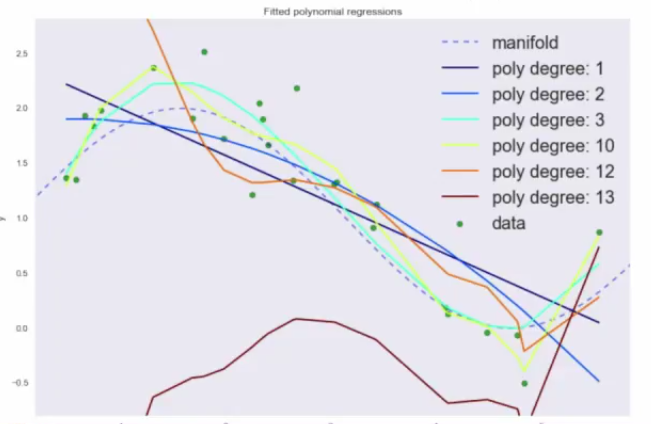
\includegraphics[scale=0.45]{polinom.png}
\caption{Съехавший полином} 
\end{figure}

Например, если вы любитель полиномов, то с вами может произойти следующая история. На рисунке \ref{pic:1} изображено несколько разных моделей. Каждая новая линия отвечает за новую модель с большим количеством степеней в правой части. При этом на 13 степени выскакивает описанная выше неадекватность. Линия, включающая в себя 13 степеней съехала куда-то вправо очень причудливым образом. Оценки коэффициентов в модели оказались искажены. 

\subsection{Мораль} 
Не забывайте думать! 
\end{document}